\documentclass[CMPE]{KGCOEReport}

\usepackage{kmap}
\usepackage{graphicx}
\usepackage{float}

\newcommand{\classCode}{CMPE 160}
\newcommand{\name}{Chris Larson}
\newcommand{\LabSectionNum}{3}
\newcommand{\LabInstructor}{Miguel Dominguez}

\newcommand{\TAs}{Andrew Ramsey \\ Madeline Mooney \\ Matthew Millar}
\newcommand{\LectureSectionNum}{2}
\newcommand{\LectureInstructor}{Professor Beato}
\newcommand{\exerciseNumber}{9}
\newcommand{\exerciseDescription}{Design and Simulation of a Moore State Machine}
\newcommand{\dateDone}{3/21/18}
\newcommand{\dateSubmitted}{3/28/18}

\begin{document}
\maketitle

\section*{Abstract}
The objective of this exercise was to design and simulate a Moore state machine based on a specific function. Multiple techniques such as developing a state transition digram, a state table, various equations and circuit diagrams were applied to design the sequential circuit. A state machine is a sequence detector. It has two inputs, an output, a clock which in this case was rising-edge-triggered, and an asynchronous active-low reset signal. The reset starts tracking the data sequence of inputs after a reset, if A = 1 and B = 1 in one clock cycle, follow by A = 1 and B = 0, and then A = 0 and B = 0, it produces an output of Z = 1. After that sequence happens if the input remains at A = 0 and B = 0, Z remains as 1; otherwise Z changes to 0, and the detector tracks the inputs until another occurrence of the sequence happens.

\section*{Design Methodology}
Using the sequence, (A,B) = (1,1),(1,0) and (0,0) then Z = 1 else Z = 0 unless (0,0) is continued after the sequence happens, a state diagram was created to demonstrate what the states would be for different situations and what situation would lead to an output of 1. The state diagram is shown in Figure 1, A is the state that the machine is in when the detector is waiting for (A,B) = (1,1), B is the state that the machine changes to when (A,B) = (1,1), C is when state B is followed by (A,B) = (1,0), D is when B is followed by C then (A,B) = (0,0) and the output is 1. It is also shown that if the machine is in state D and the input is (0,0) the output stays as 1 and the state remains D. 

\begin{figure}[H]
	\centering
	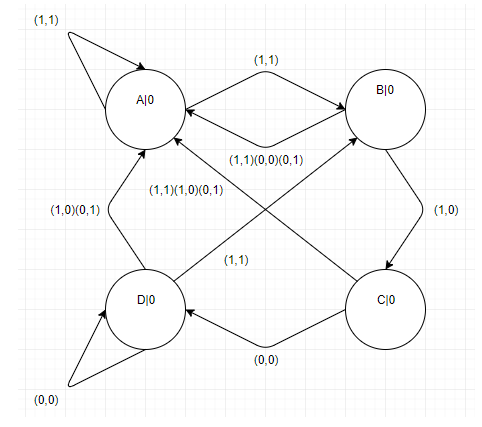
\includegraphics[width=0.6\textwidth]{StateDiagram}
	\caption{State Diagram of the machine}
	\label{fig:Figure 1}
\end{figure}

This state diagram was the basis to which the rest of the exercise follows, including a state table that shows the current, and next state as well as the output, and the equations of $Q_{1}*$ and $Q_{2}*$. The state table is shown in Table 1.

\begin{table}[H]
	\centering
	\caption{State Table for the state machine}
	\label{tab:Table 1}
	\begin{tabular}{|c|c|c|c|c|c|}
		\hline
		Current & Next(0,0) & Next(0,1) & Next(1,0) & Next(1,1) & Output(Z)\\ \hline
		00 & 00 & 00 & 01 & 00 & 0\\ \hline
		01 & 00 & 00 & 01 & 11 & 0 \\ \hline
		11 & 10 & 00 & 01 & 00 & 0 \\ \hline
		10 & 10 & 00 & 01 & 00 & 1 \\ \hline
		--  & $Q_{1} Q_{2}$ & $Q_{1} Q_{2}$ & $Q_{1} Q_{2}$ & $Q_{1} Q_{2}$ & -- \\ \hline
	\end{tabular}
\end{table}

This table was used to find the equations for $Q_{1}*$ and $Q_{2}*$ which designate which state the machine is going to be in next. A Karnuagh map was used to find the equations for $Q_{1}*$ and $Q_{2}*$ in the minimum form. The Kmaps for $Q_{1}*$ and $Q_{2}*$ are shown in Figure 2 and 3.

\begin{figure}[H]
    \centering
    \begin{Karnaugh}[A][B][Q_{1}][Q_{2}]
        \contingut{0,0,1,1,0,0,0,0,0,1,0,0,0,0,0,0} 
    	\implicant{3}{2}{red} 
    	\implicant{9}{9}{red} 
	\end{Karnaugh}
	\caption{Kmap for $Q_{1}*$ }
	\label{fig:Figure 2}
\end{figure}

The Kmap in Figure 2 yielded the equation for $Q_{1}*$ as shown in Equation 1.

\begin{equation}
	Q_{1}* = \overline{A}\,\overline{B}Q_{1} + A\overline{B}\,\overline{Q_{1}}Q_{2}
	\label{eq:Equation 1}
\end{equation}

The equation for $Q_{1}*$ shows that the next $Q_{1}*$ relies on both the current and next state. 

\begin{figure}[H]
    \centering
    \begin{Karnaugh}[A][B][Q_{1}][Q_{2}]
        \contingut{0,0,0,0,0,0,0,0,0,1,0,0,1,1,1,1} 
    	\implicant{12}{14}{red} 
    	\implicant{9}{9}{red} 
	\end{Karnaugh}
	\caption{Kmap for $Q_{2}*$ }
	\label{fig:Figure 3}
\end{figure}

The Kmap in Figure 3 yielded the equation for $Q_{2}*$ as shown in Equation 2.

\begin{equation}
	Q_{2}* = AB + A\overline{B}\,\overline{Q_{1}}Q_{2}
	\label{eq:Equation 1}
\end{equation}

The equation for $Q_{2}*$ also shows that $Q_{2}*$ relies on both the current and next state. The two equations, Equation 1 and 2, were then used to construct a circuit diagram to ensure that the equations and state diagram were correctly and performed properly. The circuit diagram uses two D flip-flops and multiple simple gates to represent the state machine, as shown in Figure 4.

\begin{figure}[H]
	\centering
	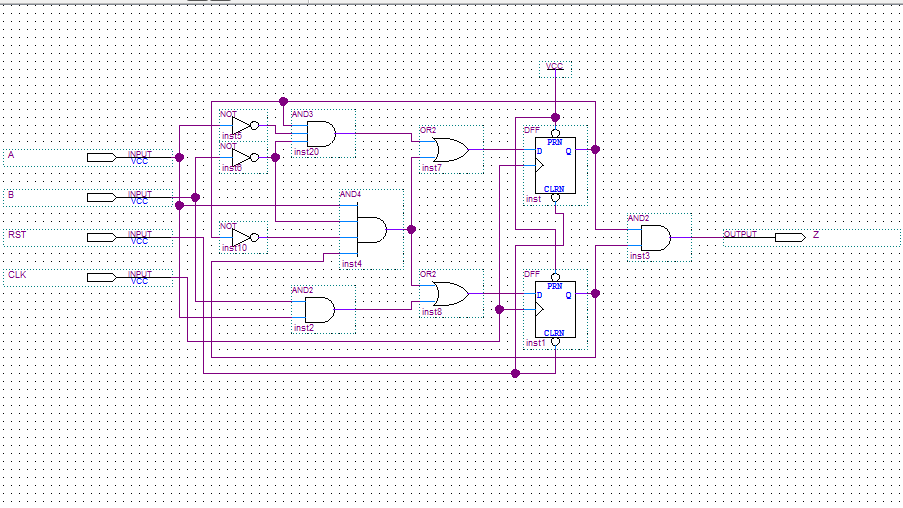
\includegraphics[width=\textwidth]{QuartusL9}
	\caption{Circuit Diagram of the machine}
	\label{fig:Figure 4}
\end{figure}

\section*{Results and Analysis}
The circuit digram shown in Figure 4 was tested using waveforms to confirm that if the specific sequence was detected that the output would change to 1, and otherwise stay at 0. Two different testbenches were used one that was premade and another that was personally created to test multiple other routes that the states could change in. The waveforms for the first testbench are shown in Figure 5 and the second testbench in Figure 6. The test sequence used in the first testbench was A=(1,1,0,1,0,1,1,0,0) and B=(1,0,0,0,0,1,0,0,0) and the sequence for the second testbench was A=(1,1,0,1,0,1,1,1,0,0) and B=(1,0,0,1,1,0,1,0,0,0).

\begin{figure}[H]
	\centering
	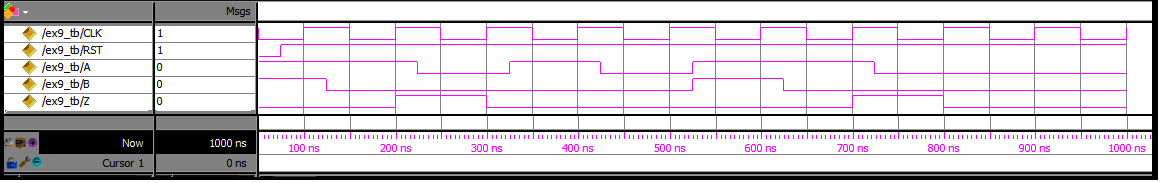
\includegraphics[width=\textwidth]{ModelSimL9}
	\caption{Waveform of the first testbench}
	\label{fig:Figure 5}
\end{figure}

The two sequences are meant to be different enough to show that the state machine did not just happen to work for one sequence and that the machine works properly according to different sequences.

\begin{figure}[H]
	\centering
	\includegraphics[width=\textwidth]{ModelSimL9PT1}
	\caption{Waveform of the second testbench}
	\label{fig:Figure 6}
\end{figure}

The circuit diagram, state table, state diagram and equations were all confirmed correct using the waveforms. The exercise was therefore a success and the state machine was created correctly.
A timing analysis was also generated during compilation and the minimum clock period and maximum clock frequency for the design were both recorded. The minimum clock period of the machine was  8.435 nanoseconds and the maximum clock frequency was 0.1186 gigahertz

\section*{Conclusion}
The use of state diagrams to turn descriptions into state machines is a very useful for real world application like vending machines and other pieces of technology that may have different states that they could be in. The exercise was a simple but effective showing of how to create and test state machines using the knowledge that has been learned previously, like karnaugh maps, circuits diagrams and confirmation by waveform. The exercise was a complete success in that the state diagram that turned into a circuit diagram functionned exactly as theorized, confirmed by the waveforms shown in Figure 5 and 6. 
\bigskip
\bigskip
\bigskip
\bigskip
\bigskip
\bigskip
\bigskip
\section*{Questions}
1.
\begin{figure}[H]
    \centering
    \begin{Karnaugh}[A][B][Q_{1}][Q_{2}]
        \contingut{0,0,1,1,0,0,0,0,0,0,1,0,0,0,0,0} 
    	\implicant{3}{2}{red} 
    	\implicant{13}{13}{red} 
	\end{Karnaugh}
	\caption{Kmap for $Q_{1}*$ }
	\label{fig:Figure 7}
\end{figure}

\begin{figure}[H]
    \centering
    \begin{Karnaugh}[A][B][Q_{1}][Q_{2}]
        \contingut{0,0,1,1,0,0,0,0,0,0,0,0,1,1,1,1} 
    	\implicant{12}{14}{red} 
    	\implicant{3}{2}{red} 
	\end{Karnaugh}
	\caption{Kmap for $Q_{2}*$ }
	\label{fig:Figure 8}
\end{figure}

\begin{table}[H]
	\centering
	\caption{State Table for the state machine}
	\label{tab:Table 1}
	\begin{tabular}{|c|c|c|c|c|c|}
		\hline
		Current & Next(0,0) & Next(0,1) & Next(1,0) & Next(1,1) & Output(Z)\\ \hline
		00 & 00 & 00 & 01 & 00 & 0\\ \hline
		01 & 00 & 00 & 01 & 10 & 0 \\ \hline
		10 & 11 & 00 & 01 & 00 & 0 \\ \hline
		11 & 11 & 00 & 01 & 00 & 1 \\ \hline
		--  & $Q_{1} Q_{2}$ & $Q_{1} Q_{2}$ & $Q_{1} Q_{2}$ & $Q_{1} Q_{2}$ & -- \\ \hline
	\end{tabular}
\end{table}

\begin{equation}
	Q_{1}* = AB + A\overline{B}\,\overline{Q_{1}}Q_{2}
	\label{eq:Equation 3}
\end{equation}

\begin{equation}
	Q_{2}* = AB + \overline{A}\,\overline{B}Q_{1}
	\label{eq:Equation 1}
\end{equation}

 \begin{figure}[H]
	\centering
	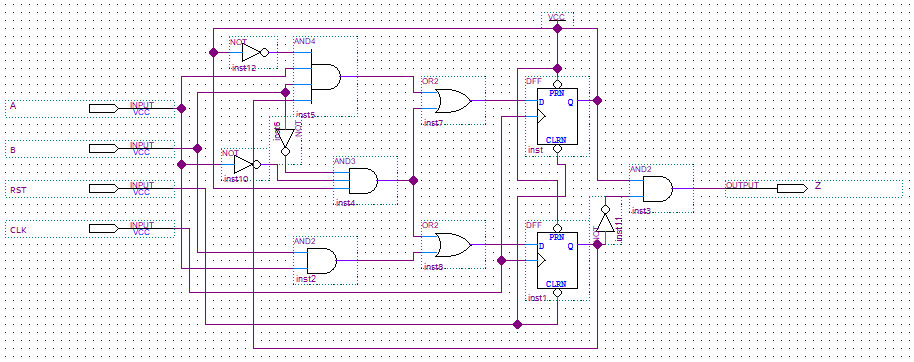
\includegraphics[width=\textwidth]{QuartusL9Q1}
	\caption{Circuit Diagram of the machine for Q1}
	\label{fig:Figure 9}
\end{figure}

This is a circuit diagram where the functionality was not in gray code, and therefore changed the kmap and equations of the state machine which in turn changes the circuit diagram.\\

2. The amount of ways to encode a state machine with four states that is implemented using two D flip-flops are 256 since the four states have four states that they could change to including themselves.\\

3. One hot encoding uses the same number of bits as there are states which lest the output logic be simpler but not very good at large design since each flip-flop is assigned a state.\\
\end{document}